\title{Arch Linuxのインストール}
\author{おがわ}
\begin{document}
  \begin{frame}
    \note {
      動画全体ので説明する項目概要です。\\
      1から4の項目があります。
    }
    \frametitle{Arch Linuxのインストール}
    \begin{enumerate}
      \item \alert<2>{ハードウェア、ファーム(UEFI)の仕様}
        \note [item] {
          ハードウェア、ファーム(UEFI)の仕様\\
          OSのインストーラソフト(Arch linux)は、ファーム(UEFI)の仕様に従いハードウェアを認識します。仕様を理解しておくと、動作しない場合の対策を立てやすくなります。
        }
      \item \alert<3>{OSのファイルシステム}
        \note [item] {
          OSのファイルシステム\\
          ストレージデバイス(ssd)のパーティション設定、各パーティションのファイルフォーマットの選定と設定をおこないます。
        }
      \item \alert<4>{Linuxのインストールと起動設定}
        \note [item] {
          Linuxのインストール\\
          インストーラソフトによるストレージデバイスへのLinuxカーネルと必要なソフトウェアのインストールを行います。インストールの後に起動設定を行います。
        }
      \item \alert<5>{ネットワークの接続設定}
        \note [item] {
          ネットワークの接続設定\\
          ネットワーク接続設定のためのソフトウェアの選定、インストールを行います。インストールの後にネットワークの設定を行います。
        }
    \end{enumerate} 
  \end{frame}
  \begin{frame}
    \frametitle{ハードウェア構成}
    \note{
      インストール対象のハードウェアは次のとおりです。
      裏面の蓋をあけて中身を確認していきます。
    }
    \newcommand{\selectspec}{\usebeamercolor[fg]{alerted text}}
    \begin{center}
      \begin{tabular}{l|l}
        \hline
        \temporal<2>{CPU}{\selectspec{CPU}}{CPU}%
          & \temporal<2>{AMD Ryzen7 8845HS}
            {\selectspec{AMD Ryzen7 8845HS}}
            {AMD Ryzen7 8845HS} \\ \hline
        \temporal<3>{メモリ}{\selectspec{メモリ}}{メモリ}%
          & \temporal<3>{64 GB}
            {\selectspec{64 GB}}{64 GB} \\  \hline
        \temporal<4>{SSD}{\selectspec{SSD}}{SSD}%
          & \temporal<4>{2 TB}{\selectspec{2 TB}}{2 TB} \\ \hline
        \temporal<5>{グラフィック}{\selectspec{グラフィック}}{グラフィック}%
          & \temporal<5>{Radeon 780M}
            {\selectspec{Radeon 780M}}
            {Radeon 780M} \\ \hline
      \end{tabular}
    \end{center}
    \begin{center}
      \includegraphics<1>[height=4cm, page=1]{img/hw-img.pdf}%
      \includegraphics<2,5>[height=4cm, page=13]{img/hw-img.pdf}%
      \includegraphics<3>[height=4cm, page=15]{img/hw-img.pdf}%
      \includegraphics<4>[height=4cm, page=14]{img/hw-img.pdf}%
    \end{center}
    \note[item]{cpuはAMD Ryzen7。本体の裏面の蓋を開けた状態の画像からは確認できません。} 
    \note[item]{memoy 32GBのメモリカード2枚で64GB}
    \note[item]{ストレージはssdで、2TBを設置}
    \note[item]{グラフィックはRadeon。こちらも画像からは確認できません。}
  \end{frame}
  \begin{frame}
    \frametitle{入出力ポート} 
    \note{
      入出力ポートについては、次のものが利用できます。
    }
    \newcommand{\selectspec}{\usebeamercolor[fg]{alerted text}}
    \begin{center}
      \begin{tabular}{l|l|l}
        \hline
        \temporal<1>{USB 3.2}{\selectspec{USB 3.2}}{USB 3.2}%
          & \temporal<1>{2}{\selectspec{2}}{2}%
          & \\ \hline
        \temporal<2>{USB 2.0}{\selectspec{USB 2.0}}{USB 2.0}%
          & \temporal<2>{2}{\selectspec{2}}{2} & \\ \hline
        \temporal<3>{HDMI}{\selectspec{HDMI}}{HDMI}%
          & \temporal<3>{2}{\selectspec{2}}{2} & \\ \hline
        \temporal<4>{DP}{\selectspec{DP}}{DP}%
          & \temporal<4>{2}{\selectspec{2}}{2} & \\ \hline
        \temporal<5>{シリアルポート}
            {\selectspec{シリアルポート}}{シリアルポート}%
          & \temporal<5>{1}{\selectspec{1}}{1}%
          & \temporal<5>{RS232、RS485}
            {\selectspec{RS232、RS485}}{RS232、RS485} \\ \hline
      \end{tabular}
      \note[item] {USB3.2タイプAのポートが2つ。位置は前面}
      \note[item] {USB2.0タイプAのポートが2つ。位置は背面}
      \note[item] {HDMIポートが2つ。位置は背面}
      \note[item] {ディスプレイポート2.1が2つ。位置は背面}
      \note[item] {シリアルのポートが1つ。位置は背面。今すぐの利用は考えていません。}
    \end{center}
    \begin{center}
      \includegraphics<1>[height=4cm, page=3]{img/hw-img.pdf}%
      \includegraphics<2>[height=4cm, page=4]{img/hw-img.pdf}%
      \includegraphics<3>[height=4cm, page=5]{img/hw-img.pdf}%
      \includegraphics<4>[height=4cm, page=6]{img/hw-img.pdf}%
      \includegraphics<5>[height=4cm, page=7]{img/hw-img.pdf}%
    \end{center}
  \end{frame}
  \begin{frame}
    \frametitle{ネットワーク} 
    \note{
      ネットワーク関連は、表のようになっています。
    }
    \newcommand{\selectspec}{\usebeamercolor[fg]{alerted text}}
    \begin{center}    
      \begin{tabular}{l|l}
        \hline
        \temporal<1>{イーサネット}{\selectspec{イーサネット}}{イーサネット}%
        & \temporal<1>{2}{\selectspec{2}}{2} \\ \hline
        \temporal<2>{Wi-Fi}{\selectspec{Wi-Fi}}{Wi-Fi}%
        & \temporal<2>{1}{\selectspec{1}}{1}\\
        \hline
      \end{tabular}
      \note[item] {イーサネットポートが2つ。位置は背面}
      \note[item] {Wi-Fiが1つ。アンテナが背面に確認できます}
    \end{center}
    \begin{center}
      \includegraphics<1>[height=4cm, page=8]{img/hw-img.pdf}%
      \includegraphics<2>[height=4cm, page=9]{img/hw-img.pdf}%
    \end{center}
  \end{frame}
  \begin{frame}
    \frametitle{ファーム}
    \note{
      AMI社のファームで、UEFI仕様に従っています。
      起動ボタン押下直後にF2で設定が変更できます。
      ファームについて簡単な説明をしておきます。
      ファームとはマザーボードのチップに書き込まれたソフトウェアです。ファームは、CPUやマザーボードに接続された機器との通信を行います。ファームは、基本的な機能だけを提供しています。ファームの機能を組み合わせて利用すると複雑な処理を行うことができます。\\
      ファームがUEFI仕様に従っているおかげで、汎用的にソフトウェアを開発することができます。
      このことについて、次に説明していきます。
    }
    \begin{center}
    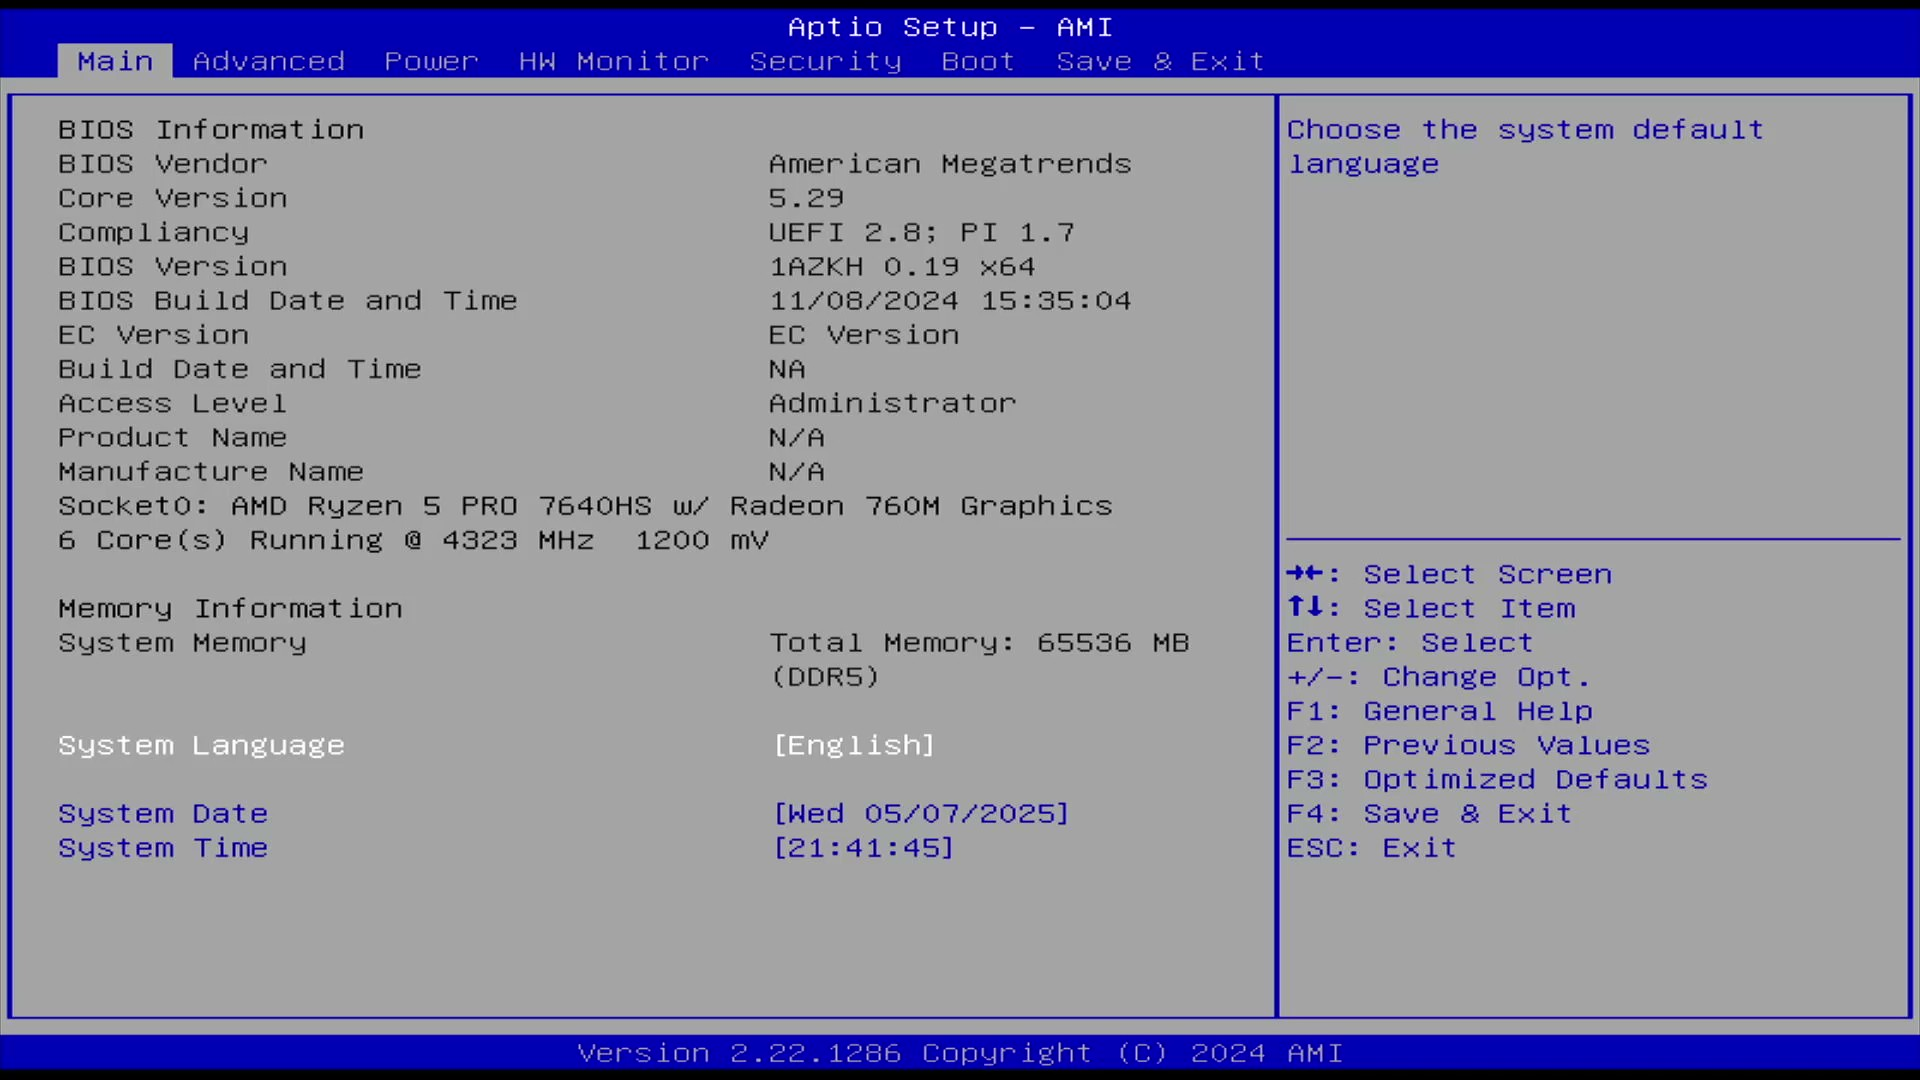
\includegraphics[height=5cm]{img/bios-display-1.jpg}
    \end{center}
  \end{frame}
  \begin{frame}
    \frametitle{要件を満たすソフトウェア}
    \note{ファームの説明のために、ユーザーの要件を満たすようなソフトウェアを開発することを考えます。}
    \only<1>{要件\\}%
    \only<2>{開発\\}%
    \only<3>{査収\\}%
    \only<4>{運用\\}%
    \only<5>{改修要件\\}%
    \only<6>{改修\\}%
    \only<7>{ソフト移行\\}%
    \begin{center}
      \includegraphics<1>[height=6cm, page=1]{img/sw-requirement.pdf}%
      \includegraphics<2>[height=6cm, page=2]{img/sw-requirement.pdf}%
      \includegraphics<3>[height=6cm, page=3]{img/sw-requirement.pdf}%
      \includegraphics<4>[height=6cm, page=4]{img/sw-requirement.pdf}%
      \includegraphics<5>[height=6cm, page=5]{img/sw-requirement.pdf}%
      \includegraphics<6>[height=6cm, page=6]{img/sw-requirement.pdf}%
      \includegraphics<7>[height=6cm, page=7]{img/sw-requirement.pdf}%
    \end{center}
    \note[item]<1>{発注者の要件を明確にします。}
    \note[item]<2>{要件を元に、ソフトウェアを開発します。
      通常は、成果物、設計、納期、テストケースなどについても、発注者と確認を取ります。ここでは割愛しています。}
    \note[item]<3>{発注者が、要件をみたしていることを確認して、受領となります。}
    \note[item]<4>{受領されたソフトウェアの運用を開始します。ここでは、発注者が運用していますが、運用は別の組織となることも多いです。}
    \note[item]<5>{実運用を始めると、当初の要件では、気付かなかった問題が生じることがあります。iPhoneアプリの応答が遅いとか\ldots  このケースでは、サーバの処理能力の向上で解決する追加要件となっています。}

    \note[item]<6>{要件を満たすサーバを選定します。}
    \note[item]<7>{現行サーバのソフトについて、新サーバでも動作させることができるのでしょうか?}  
  \end{frame}
  
  \begin{frame}
    \frametitle{ハードウェアの利用とソフトウェア}
    \alt<2>{UEFIがある}{UEFIがない}
    \includegraphics<1>[height=4cm, page=1]{img/hw-fm-sw.pdf}%
    \includegraphics<2>[height=4cm, page=2]{img/hw-fm-sw.pdf}%
    \note{ハードウェアがそれぞれ、異なる形式で機能を提供すると、利用する側もハードウェアの種類だけ必要になってしまいます。統一した形式で、機能を提供することで、複雑な処理を行う側が、1種類で済むようになります。この統一した仕様としてUEFIがあります。}

  \end{frame}

  \begin{frame}
    \frametitle{iPXEのダウンロード}
    以下のURLのページからUEFI用のiPXEをダウンロード\\
    \url{https://archlinux.org/releng/netboot/}\\
    \begin{center}
      \includegraphics<1>[bb=0 2cm 6cm 8.61cm,clip=true, height=4cm, page=1]
        {img/ipxe-http-page.pdf}%
      \includegraphics<2>[bb=0 2cm 6cm 8.61cm,clip=true, height=4cm, page=2]
        {img/ipxe-http-page.pdf}%
      \includegraphics<3>[bb=0 2cm 4cm 5cm,clip=true, height=4cm, page=1]
        {img/ipxe-http-page.pdf}%
      \includegraphics<4>[bb=0 2cm 4cm 5cm,clip=true, height=4cm, page=3]
        {img/ipxe-http-page.pdf}%
    \end{center}
    \uncover<4->{\url{https://archlinux.org/static/netboot/ipxe-arch.efi}}
  \end{frame}
  \begin{frame}
    \frametitle{Netboot用USB作成}
    \begin{enumerate}
      \item<1-> USBのドライブにEFI{\textbackslash}BOOTディレクトリを作成する
      \item<2-> ipxe-arch.efiをBOOTx64.efiに変名する
      \item<3-> BOOTx64.efiをEFI{\textbackslash}BOOTに保存する
    \end{enumerate} 
    \note{
      UEFIの仕様ではUSBフラッシュがFAT8、FAT16、FAT32のファイルシステムで、EFI{\textbackslash}BOOT.EFIがUEFIアプリケーション(BOOT loader)として認識されます。
      動画では、ipxe-arch.efiはipxe-archの後ろに16進数が続いていますが、最近のarch用のipxeのダウンロードでは、16進数がつかないようです。
    }
  \end{frame}

\end{document}
% vi: se ts=2 sw=2 et:
